\documentclass[11pt,a4paper]{article}
\usepackage[T1]{fontenc}
\usepackage{lmodern}
\usepackage[margin=2.5cm]{geometry}
\usepackage{amsmath,amssymb}
\usepackage{booktabs}
\usepackage{graphicx}
\usepackage{listings}
\usepackage{xcolor}
\usepackage[hidelinks]{hyperref}

\newcommand{\code}[1]{\texttt{#1}}
\newcommand{\bn}{\mathbf{n}}
\newcommand{\bx}{\mathbf{x}}
\newcommand{\bu}{\mathbf{u}}
\lstset{basicstyle=\ttfamily\small, breaklines=true, columns=fullflexible, keepspaces=true, frame=single,
        framerule=0.3pt, rulecolor=\color{gray}, xleftmargin=1em, xrightmargin=1em,
        literate={ψ}{{$\psi$}}1 {Ω}{{$\Omega$}}1 {θ}{{$\theta$}}1 {ρ}{{$\rho$}}1 {r̂}{{$\hat r$}}1
                 {×}{{$\times$}}1 {⋅}{{$\cdot$}}1 {λ}{{$\lambda$}}1 {φ}{{$\varphi$}}1}

\title{The \code{Polyhedral} submodule of \code{dmplex}:\\ user documentation and test examples}
\author{Oswald Knoth}
\date{\today}

\begin{document}
\sloppy
\maketitle

\begin{abstract}
\code{dmplex.Polyhedral} carries the finite-volume method of the Fortran code POLYEDER over to
Julia: cell complexes of general polyhedra, the exact integration of monomials over cells and faces,
an average-preserving polynomial reconstruction, upwind transport, face gradients from interaction
regions, the shallow-water equations on one layer of cells over the sphere (KernelAbstractions, MPI,
GPU), and cut cells over orography. This document describes how the pieces are used and shows the
results of the test examples. The derivations are in the companion paper draft
\code{docs/polyhedral/polyhedral.tex}.
\end{abstract}

\tableofcontents

%==============================================================================
\section{Overview}

\begin{table}[h]
\centering\small
\begin{tabular}{ll}
\toprule
file (\code{src/Polyhedral/}) & contents \\
\midrule
\code{Complex.jl} & \code{PolyComplex}, \code{extruded\_complex}, \code{face\_cells}, \code{vertex\_neighbours} \\
\code{Integration.jl} & \code{MonomialBasis}, \code{cell\_moments}, \code{face\_moments}, \code{face\_quadrature} \\
\code{Geometry.jl} & \code{PolyGeometry}: volumes, centroids, areas, normals \\
\code{Reconstruction.jl} & \code{PolyReconstruction}, \code{face\_value\_matrices}, \code{point\_value\_matrices} \\
\code{Advection.jl} & \code{PolyAdvection}, \code{stream\_function\_flux}, \code{vector\_potential\_flux} \\
\code{InteractionRegion.jl} & \code{interaction\_operators}, \code{cell\_vectors}, \code{linear\_vector\_reconstruction} \\
\code{ShallowWater.jl} & \code{PolyShallowWater}: kernels, MPI distribution, time step \\
\code{CutCell.jl} & \code{cut\_complex}, \code{merge\_cells}, \code{merge\_small\_cells} \\
\code{Euler.jl} & \code{PolyEuler}: compressible Euler equations on extruded cells, IMEX \\
\bottomrule
\end{tabular}
\caption{Files of the submodule.}
\end{table}

The data flow is the same for every application: a \code{PolyComplex} (from an \code{ExtrudedPlex}
or cut by a surface), its \code{PolyGeometry}, operators assembled once as sparse matrices
(reconstruction, face values, gradients), and a \code{tendency!(dy, y, model)} for the explicit
time steppers of \code{dmplex} (\code{SSPRK3Cache}, \code{ssprk3\_step!}). All functions are in the
module \code{dmplex.Polyhedral}; the exported ones are listed in \code{Polyhedral.jl}, the others are
reached as \code{dmplex.Polyhedral.name} (below \code{PH.name}).

%==============================================================================
\section{Cell complexes}\label{sec:complex}

A \code{PolyComplex} stores cells, faces, edges and vertices, numbered from 1 in each dimension,
with compressed cones and incidence numbers $\pm 1$:
\begin{itemize}
\item the faces of cell $c$ are \code{cell\_faces[cell\_offsets[c]:cell\_offsets[c+1]-1]}, with
  \code{cell\_signs} $+1$ when the face normal points out of the cell;
\item the edges of a face, likewise in \code{face\_offsets}, \code{face\_edges}, \code{face\_signs}, the
  orientation of the face (and so its normal) given by the edge loop;
\item \code{edge\_vertices} ($2\times$edges, $\partial e = v_2 - v_1$) and \code{coordinates}.
\end{itemize}
\code{PH.cell\_cone(cx, c)} and \code{PH.face\_cone(cx, f)} return the cone and its signs,
\code{PH.face\_loop(cx, f)} the vertices of a face in order. \code{face\_cells(cx)} gives the two cells
of every face ($2\times$faces): the one the normal points out of, then the one it points into, $0$ on
the boundary. Faces need not be planar: a non-planar face is integrated over the fan of triangles
from its vertex mean (\code{planar\_pieces}).

The complexes used so far are prisms over a 2D mesh:
\begin{lstlisting}
using dmplex
plex = create_hexagon_mesh(3)    # or create_spherical_mesh(3), create_cubed_sphere_mesh(8)
cx   = extruded_complex(ExtrudedPlex(plex, 1), [0.0, 1000.0]; radius=6.37122e6)
geo  = PolyGeometry(cx)                     # volume, cell_centroid, area, normal, face_centroid
\end{lstlisting}
On the sphere vertex $v$ of level $k$ is at $(R + z_k)\,v$, on a plane at $v + z_k\,\hat z$; a plane
mesh comes from \code{plex\_from\_polygons(polygons, points)}. Figure~\ref{fig:meshes} shows one layer
over the three spherical meshes of the tests.

\begin{figure}[t]
\centering
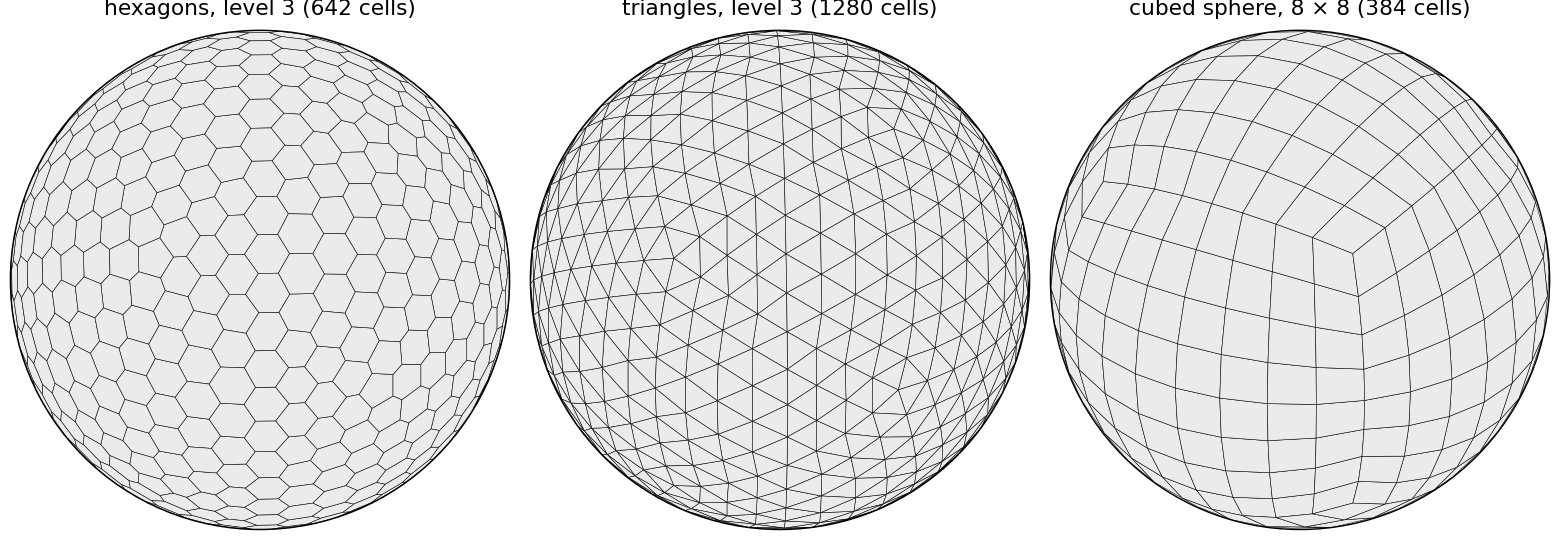
\includegraphics[width=\textwidth]{figures/poly_meshes.png}
\caption{One layer of prisms over the sphere: the bottom faces of the hexagonal, the icosahedral
(triangles) and the cubed-sphere mesh.}\label{fig:meshes}
\end{figure}

%==============================================================================
\section{Moments and geometry}

\code{MonomialBasis(p)} lists the exponents $\alpha$ of the monomials $y^\alpha$ of degree $\le p$
in three variables. \code{cell\_moments(cx, c, B; center, scale, rotation)} returns the integrals
$\int_C y^\alpha\,dV$ in the local coordinates $y = Q(\bx - \bx_0)/h$, exactly, by homogeneous
integration down the cone hierarchy (cell $\to$ faces $\to$ edges $\to$ vertices);
\code{face\_moments} does the same for a face. Without \code{center} and \code{scale} a frame of the
cell (or face) itself is used, which keeps the recursion well conditioned. \code{PolyGeometry} takes
volumes and centroids from the moments of degree~$\le 1$, the unit normal of a face from its area
vector. \code{face\_quadrature(cx, f)} gives points and area vectors of a rule of degree~5 on a face
(the seven-point rule on every triangle of the fan).

The test set ``cell complexes and the integration of monomials'' checks the moments against exact
values on the unit cube, a triangular prism and a non-convex L-shaped prism, in shifted and scaled
frames, the divergence theorem for every monomial, the closure $\sum_F s_{CF}|F|\bn_F = 0$ and the
volume of a spherical shell over icosahedra, and the closure of hexagonal prisms with non-planar
faces.

%==============================================================================
\section{Reconstruction and transport}\label{sec:transport}

\subsection{Reconstruction}
\begin{lstlisting}
rec = PolyReconstruction(cx, geo, degree; basis=:full, rings=nothing,
                         oversampling=1.5, boundary_oversampling=oversampling,
                         up=normalize, rtol=1e-8)
Q1, Q2 = face_value_matrices(cx, rec)     # faces x cells: face averages of side 1 and 2
reconstruct(rec, c, u, x)                  # value of the polynomial of cell c at x
\end{lstlisting}
For every cell the polynomial of degree \code{degree} that has the cell average and fits the
averages of the stencil in the least-squares sense. The stencil grows by vertex rings until the
problem has full rank and \code{oversampling} times as many cells as monomials;
\code{boundary\_oversampling} is used for the cells with a boundary face, whose stencils are
one-sided (the cut cells at the terrain need $2.5$ for degree~2). \code{basis=:tangential} drops
the monomials in the direction \code{up(x\_C)}: the reconstruction in the tangent plane for one layer
over the sphere. The coefficients are linear in the averages, so face values and point values are
sparse matrices (\code{face\_value\_matrices}, \code{point\_value\_matrices}).

\subsection{Transport}
\begin{lstlisting}
U = stream_function_flux(cx, ψ; G=r -> r^3/3)   # volume fluxes through the faces
m = PolyAdvection(cx, U; degree=2, basis=:tangential)
dt = 0.4 * upwind_time_step(m)
cache = SSPRK3Cache(q)
ssprk3_step!(q, dt, PH.tendency!, cache, m)
\end{lstlisting}
\code{PolyAdvection(cx, flux)} transports cell averages with the upwind face averages of the
reconstruction; with a velocity function instead of the fluxes it integrates $(\bu\cdot\bn)\,q$ at the
quadrature points of the faces, each point upwinded, which gives the order of the reconstruction
(degree 3: order 4 in the test). Divergence-free fluxes come from a potential:
\code{stream\_function\_flux(cx, $\psi$; G, height, project)} for $\bu = g(h)\nabla\psi\times\nabla h$ on
the sphere (solid-body rotation: $\psi = \Omega\cdot\hat r$, $G(r) = r^3/3$; with the default
$G(r) = r$ the rotation on a shell $1\le r\le 1.01$ is about $1\,\%$ too slow), and
\code{vector\_potential\_flux(cx, A)} for $\bu = \nabla\times A$ in general, the circulation of $A$
around every face. In both cases the outward fluxes of every cell sum to zero to round-off.

Figure~\ref{fig:rotation} shows a Gaussian hill $q = \exp(-|\hat r - \hat x|^2/0.16)$ after one
revolution about the axis $(1,0,1)/\sqrt 2$ on hexagons of level~5 (10242 cells). The relative
$L^2$ errors are $0.120$, $0.033$ (degree~1) and $0.120$, $0.022$ (degree~2) on levels 4 and 5; mass
is conserved to $10^{-13}$.

\begin{figure}[t]
\centering
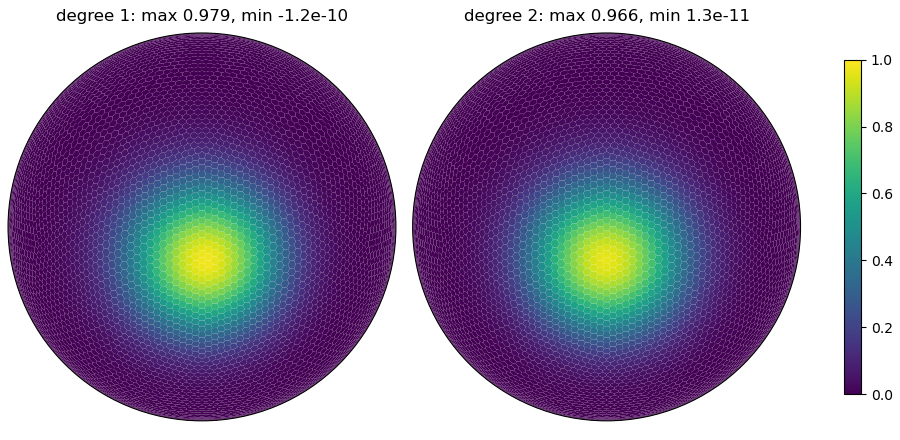
\includegraphics[width=0.8\textwidth]{figures/poly_rotation.png}
\caption{Solid-body rotation of a Gaussian hill on hexagons, level 5, after one revolution
(587 steps of SSP-RK3), degree 1 and 2 of the reconstruction.}\label{fig:rotation}
\end{figure}

%==============================================================================
\section{Interaction regions and cell vectors}

\begin{lstlisting}
G, T = interaction_operators(cx, geo)   # faces x cells: normal gradient, face value
vc  = cell_vectors(cx, geo, un)         # Perot: vector at the cells from normal components
R   = cell_vector_matrices(cx, geo)     # the same as three sparse matrices
R   = linear_vector_reconstruction(cx, geo; own_weight=20)   # linear fit, second order
un  = face_normal_components(cx, geo, vc)
\end{lstlisting}
Around every vertex the cells and faces meeting there form an interaction region (POLYEDER
\code{TGrad}); a gradient per cell, continuous normal components across the faces of the region,
gives the normal gradient \code{G} and the face value \code{T} as sparse matrices, exact for linear
fields at faces away from the boundary. \code{cell\_vectors} is Perot's reconstruction
$v_C = |C|^{-1}\sum_F s_{CF}|F|\,u_F\,(\bx_F - \bx_C)$, exact for constant fields only;
\code{linear\_vector\_reconstruction} fits a linear field to the normal components of the cell and
its neighbours (own faces weighted by \code{own\_weight}) and is second order on triangles as well.

%==============================================================================
\section{Shallow water on one layer}

\begin{lstlisting}
m = PolyShallowWater(cx; gravity=9.80616, omega=7.292e-5, bathymetry=nothing,
                     degree=2, cell_vector=:auto, comm=nothing, backend=CPU())
y = initial_state(m, velocity, height)       # local [h; U], U = h u.n at the faces
dt = shallow_water_time_step(m, y; cfl=0.4)
cache = SSPRK3Cache(y)
ssprk3_step!(y, dt, tendency!, cache, m)
state = gather_state(m, y); total_mass(m, y); M = cell_momentum!(m, y)
\end{lstlisting}
Heights are cell averages, momenta normal components at the faces. The pressure gradient comes from
\code{interaction\_operators}, advection and Coriolis act on the cell momentum (Perot, or the linear
fit: \code{cell\_vector=:linear}, chosen by \code{:auto} on triangular prisms), whose Cartesian
components are transported with the upwind face values of the reconstruction and projected back to
the faces. All terms are KernelAbstractions kernels over padded tables; with \code{backend =
CUDABackend()} they run on the GPU. With an MPI communicator \code{comm} the cells are partitioned by
area, ghosts are the stencil columns of the owned rows, and the result is bitwise equal to the serial
run (test \code{test/mpi\_poly.jl}, 1 and 3 ranks).

\paragraph{Galewsky et al.\ (2004).} \code{examples/polyhedral/galewsky\_poly.jl}, configured by
environment variables (\code{MESH=icosahedral|hexagonal|cubed LEVEL DAYS CV PERTURB GPU OUT}), runs the
barotropic jet; on Levante one A100 per case (\code{poly\_galewsky.sbatch}, set
\code{SLURM\_CPUS\_PER\_TASK=16}). Six days at level 7 take 1--2 minutes on the GPU, the setup of the
operators on the host 10--14 minutes. Figure~\ref{fig:galewsky} shows the relative vorticity at day 6.
The perturbed jet rolls up as expected on all three meshes; the unperturbed jet should stay zonal,
but breaks up into waves of the grid's wavenumber~5 by day~6: the open problem of the one-layer model.
The pressure gradient of the interaction regions is first order in the maximum norm near the
irregular vertices (second order in the mean), the current suspect.

\begin{figure}[p]
\centering
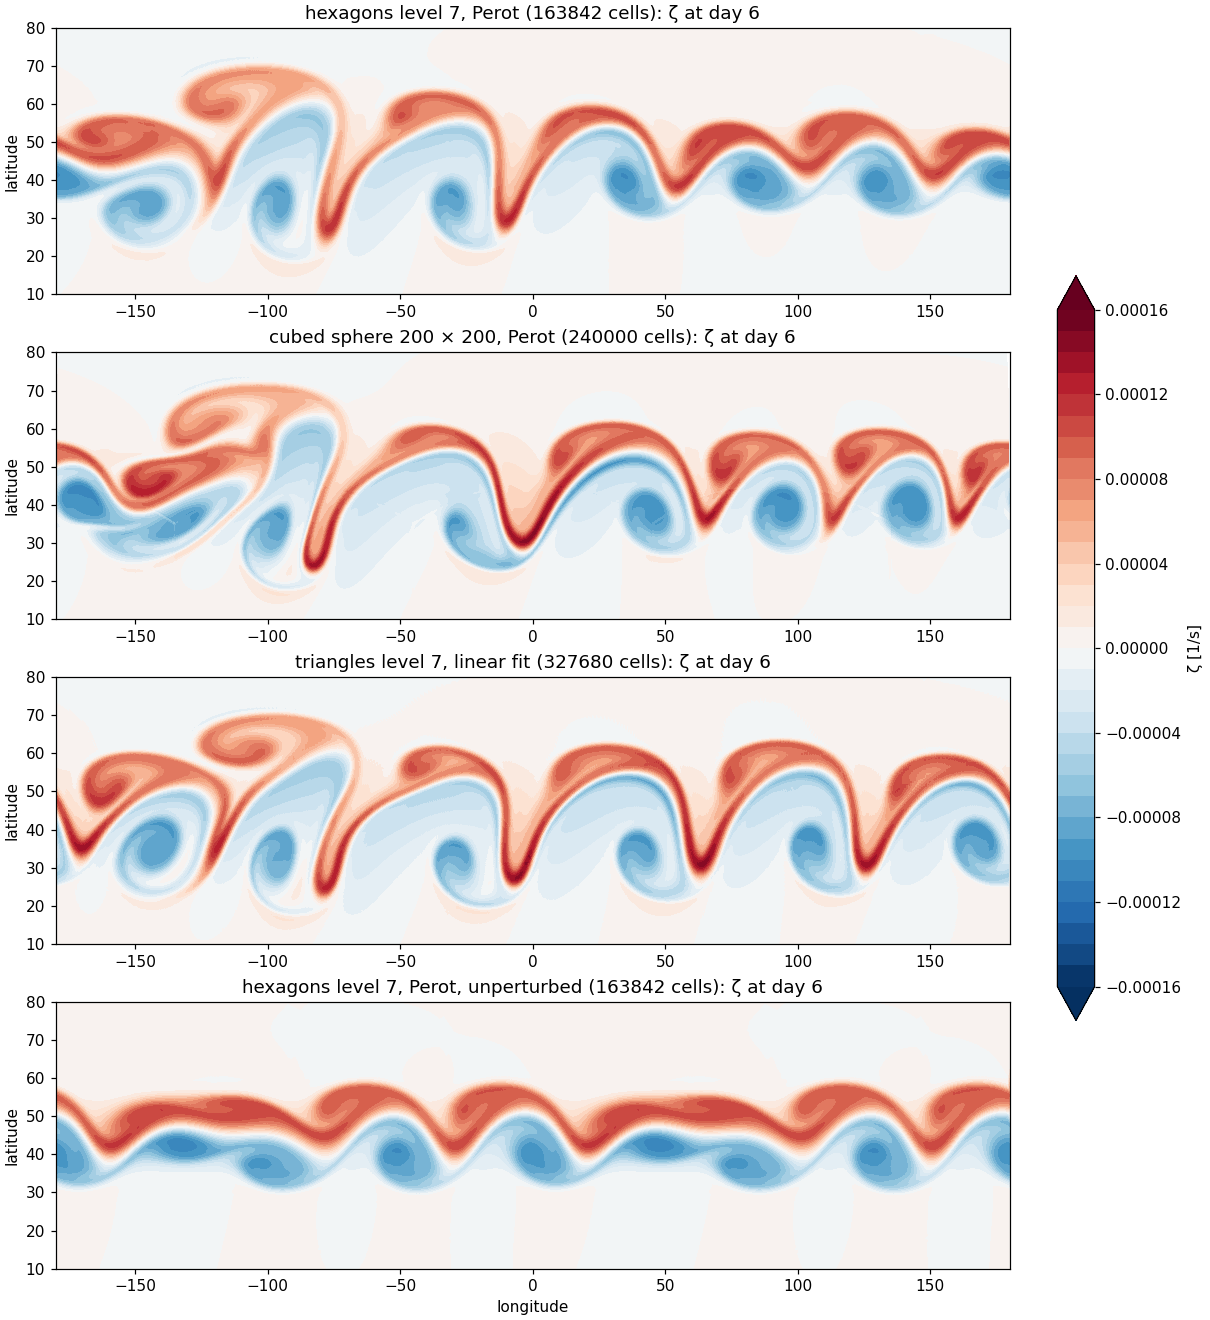
\includegraphics[width=0.95\textwidth]{figures/poly_galewsky.png}
\caption{Galewsky test, relative vorticity at day 6: perturbed jet on hexagons (Perot), the cubed
sphere ($200\times 200$ per face, Perot) and triangles (linear fit), and the unperturbed jet on
hexagons.}\label{fig:galewsky}
\end{figure}

%==============================================================================
\section{Cut cells}\label{sec:cut}

\begin{lstlisting}
level(x) = x[3] - zs(x[1], x[2])                 # > 0 in the fluid
cut, parent, terrain = cut_complex(cx, level)   # parent cell, terrain faces
g0 = PolyGeometry(cx)
merged, group = merge_small_cells(cut, g0.volume[parent]; fraction=0.5)
\end{lstlisting}
\code{cut\_complex} follows POLYEDER's \code{CutGrid}: vertices with \code{level < 0} are removed,
edges between the fluid and the ground are cut at the root of \code{level} (Illinois method), every
cut face is closed by the edge between its two cut points, every cut cell by a terrain face through
these edges (non-planar in general, oriented outward). A face crossed twice by the surface, or a
vertex exactly on it, is an error. \code{merge\_small\_cells} unites every cell smaller than
\code{fraction} times its reference volume with the neighbour across its largest face, repeatedly;
\code{group} maps the cut cells to the merged ones, and a merged cell is again a polyhedron of the
complex, so moments, reconstruction and transport apply unchanged.

The test (Figure~\ref{fig:cut}) cuts jittered triangular prisms over
$[-1,1]\times[0,\tfrac14]\times[0,1]$ by $z_s = 0.03 + 0.25\,e^{-(x/0.4)^2}\cos^2(\pi x/0.5)$. Unmerged,
the smallest cell has $2.5\cdot10^{-11}$ of its prism (inside the domain, not on the wall shown); merged
at $0.5$ the steady transport $q = e^{2\psi}$ by $\bu = \nabla\times(\psi\hat y)$, $\psi = 0$ on the
terrain and the top, runs with 26 instead of 74638 steps on $16\times8$ and converges with orders
$1.76$ and $1.91$ ($16\times8 \to 32\times16 \to 64\times32$).

\begin{figure}[t]
\centering
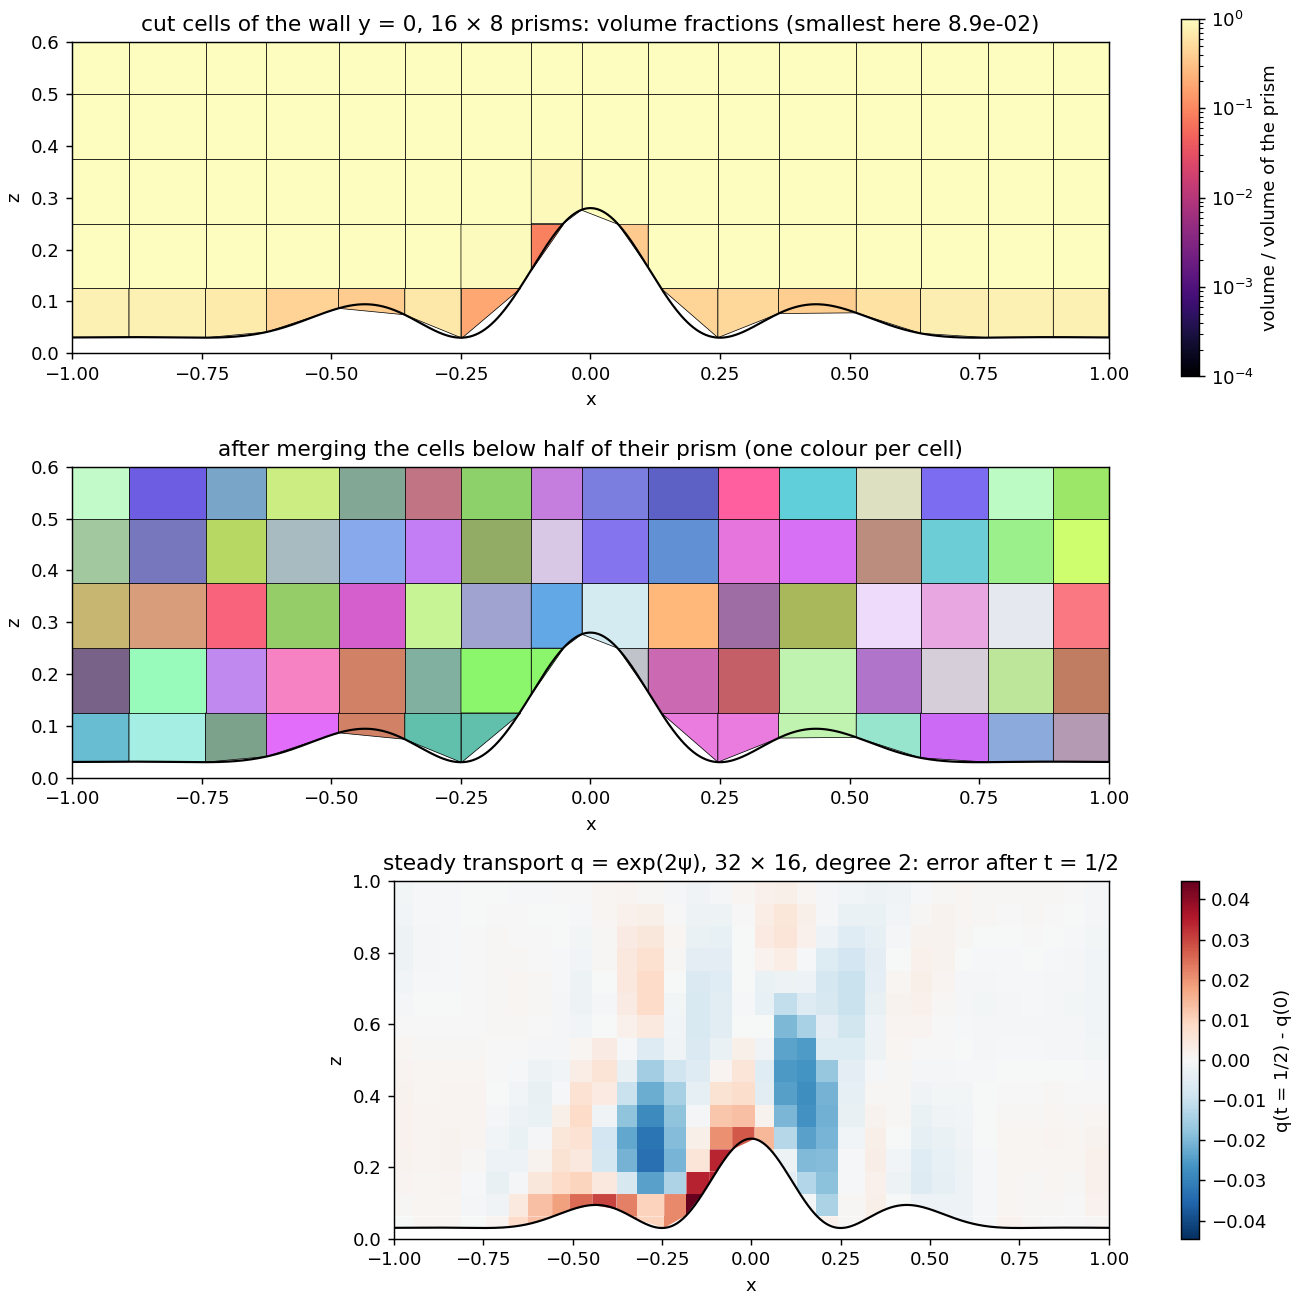
\includegraphics[width=0.85\textwidth]{figures/poly_cut.png}
\caption{Cut cells on the wall $y = 0$ of the test: volume fractions of the cut cells ($16\times8$),
the cells after merging, and the error of the steady transport ($32\times16$, degree 2,
$t = 1/2$).}\label{fig:cut}
\end{figure}

\subsection{Flow over a hill on a Cartesian cut-cell grid}\label{sec:mountain}

\code{examples/polyhedral/mountain.jl} solves the compressible Euler equations on a Cartesian grid of
hexahedra (one cell across in $y$) cut by the hill and merged at $0.5$. Prognostic are the cell
averages of $\rho$ and $\rho\theta$ and the normal momentum $M_F = (\rho\bu)\cdot\bn_F$ at the faces
(a C grid; zero at the terrain, the top and the side walls, prescribed at the lateral boundaries):
\begin{align*}
\partial_t\rho_C &= -|C|^{-1}\textstyle\sum_F s_{CF}|F|M_F, \qquad
\partial_t(\rho\theta)_C = -|C|^{-1}\textstyle\sum_F s_{CF}|F|M_F\,\theta_F^{\uparrow},\\
\partial_t M_F &= \bn_F\cdot\big(w_1 A_{C_1} + w_2 A_{C_2}\big)
  - \frac{p'_{C_2} - p'_{C_1}}{\bn_F\cdot(\bx_{C_2} - \bx_{C_1})} - g\,n_{F,z}\,\big(w_1\rho'_{C_1} + w_2\rho'_{C_2}\big)
  - \tau_F\,(M_F - M_F^0),
\end{align*}
with $p = p_{00}(R_d\rho\theta/p_{00})^{\gamma}$, the perturbations $p'$, $\rho'$ against the
discrete initial state at rest (which is therefore exactly balanced),
$A_C = -|C|^{-1}\sum_F s_{CF}|F|M_F\,\bu_F^{\uparrow}$ the momentum advection of the cell velocity
$\bu_C = m_C/\rho_C$ (Perot's $m_C$), $\uparrow$ the upwind face values of the degree-2
reconstruction, $w_{1,2}$ the linear interpolation weights along the normal, and Rayleigh damping
$\tau$ above $z_D$ and near the lateral boundaries. The initial flow is the discrete curl of
$A = -\psi\hat y$ with $\psi = U_0\,[\,R(z) - R(z_s)\max(0, (z_d - z)/(z_d - z_s))\,]$,
$R(z) = \int_0^z \rho_0$, $z_d = 5$~km: divergence free, tangential to the terrain, uniform aloft.
SSP-RK3 with the acoustic time step.

The test of Gallus and Klemp (2000): Agnesi hill $h(x) = h_0/(1 + (x/a)^2)$, $h_0 = 400$~m,
$a = 1$~km, $U_0 = 10$~m/s, $N = 0.01$~s$^{-1}$ ($Na/U_0 = 1$, nonhydrostatic, $Nh_0/U_0 = 0.4$),
$\theta_s = 300$~K, $\Delta x = 250$~m, $\Delta z = 125$~m. Figure~\ref{fig:mountain} compares $w$ and
$\theta'$ with the linear solution (Fourier integral with radiation condition and the amplitude
growth $\sqrt{\rho_0(0)/\rho_0(z)}$).
The domain is $50 \times 20$~km ($200\times160$ Cartesian cells, 31970 after cutting and
merging), with damping above $12$~km and beyond $|x| = 17$~km; $\Delta t = 0.152$~s, 71276 steps for
3~h, 68 minutes on 8 threads of a Mac mini. At $t = 3$~h the maximum of $|w|$ is $2.36$~m/s
(linear $2.40$), at $z = 2$~km $w$ lies between $-1.36$ and $0.89$~m/s (linear $-1.33$, $0.92$), and
the phase lines of $w$ and $\theta'$ follow the linear solution; the isentropes pass smoothly over the
hill, without noise from the cut cells. The mass changes by less than $2\cdot10^{-5}$, only through the
relaxation in the damping layers.

\begin{figure}[t]
\centering
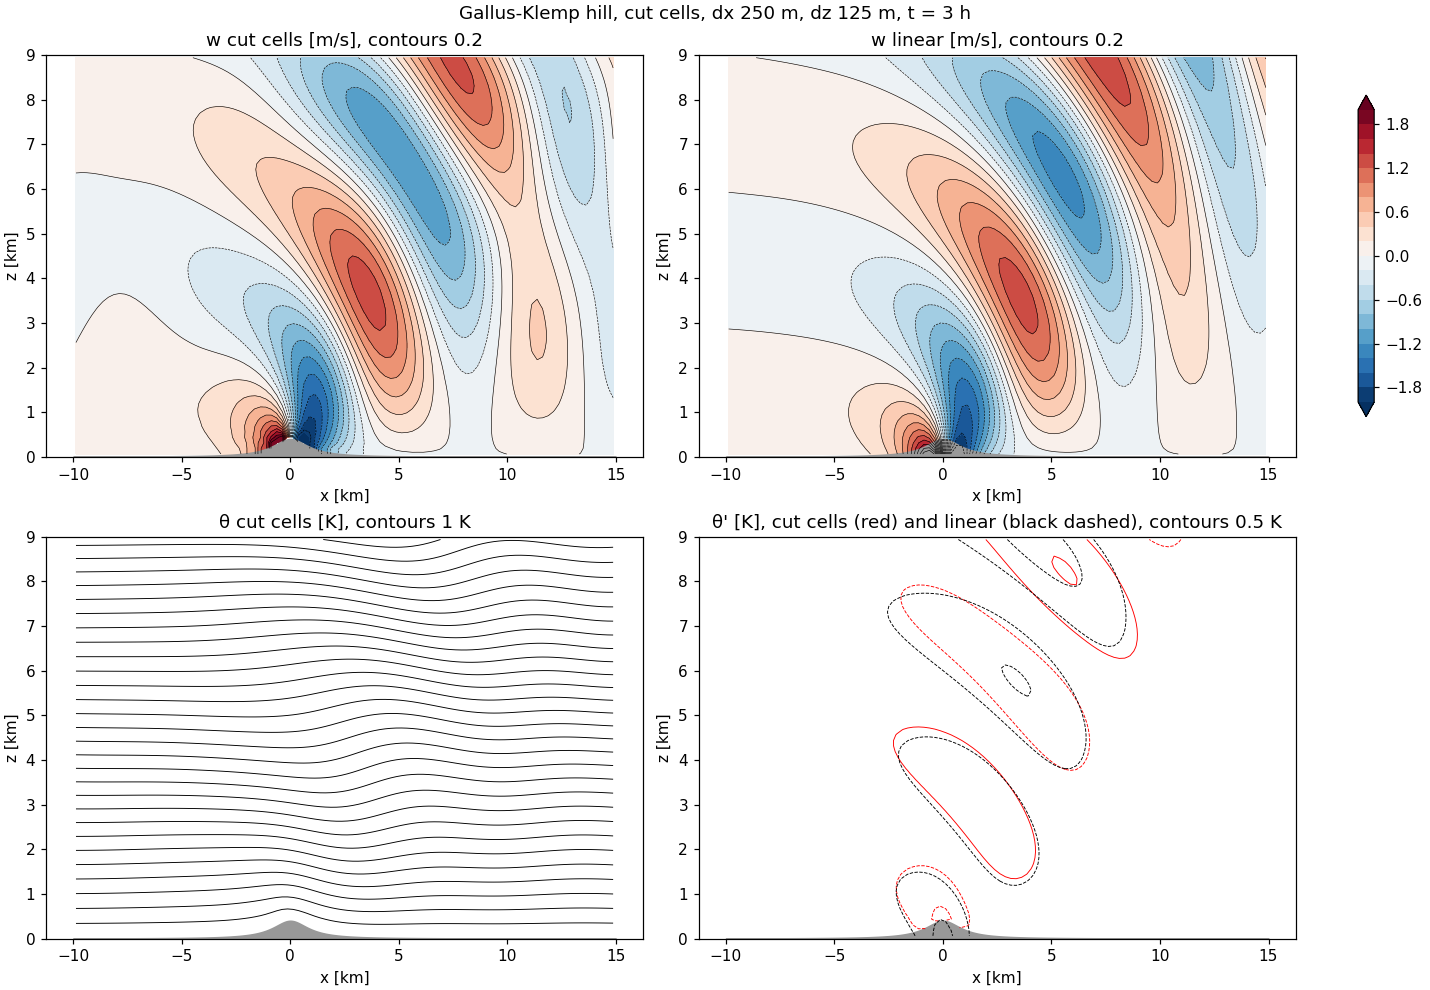
\includegraphics[width=\textwidth]{figures/poly_mountain.png}
\caption{Flow over the Gallus--Klemp hill on the Cartesian cut-cell grid: $w$ of the model and of the
linear solution, $\theta$, and $\theta'$ of the model (red) and the linear solution (black dashed).}
\label{fig:mountain}
\end{figure}

%==============================================================================
\section{The Euler equations on extruded cells}\label{sec:euler}

\begin{lstlisting}
v  = VerticalGrid(30, 30000.0)
cx = extruded_complex(ExtrudedPlex(create_hexagon_mesh(5), 30), v.z_half; radius=6.37122e6)
m  = PolyEuler(cx, v.z_half; radius=6.37122e6, damping_height=22000.0, damping_rate=0.05,
               degree=1, projection=:adjoint)
y  = initial_state(m, (λ, φ, z) -> baroclinic_wave(λ, φ, z))
ys = zero_state(m)
step!(m, y, 300.0, ys)
surface_pressure(m, y); lowest_temperature(m, y); vertical_velocity(m, y); total_mass(m, y)
\end{lstlisting}
\code{PolyEuler} is the mountain scheme of Section~\ref{sec:mountain} on the prisms of an
\code{extruded\_complex}, over the sphere or the plane: $\rho$ and $\rho\theta$ at the cells, the normal
momentum $M_F$ at the faces, $\theta$ and the velocity upwind from the reconstruction of degree
\code{degree}, the pressure gradient between the two cells along the normal and the buoyancy of the
deviations $p'$, $\rho'$ from an isothermal state at rest. It has the interface of the other dycores
(\code{initial\_state(m, profile)}, \code{zero\_state}, \code{step!}, \code{total\_mass},
\code{surface\_pressure}, \code{lowest\_temperature}, \code{vertical\_velocity}), so the test cases of
\code{Nonhydrostatic} run with it through \code{examples/dycores.jl} (\code{baroclinic\_wave.jl poly},
\code{thermal\_wind.jl poly}). Four choices were needed for the baroclinic wave:

\begin{enumerate}
\item \emph{Heights from the levels.} The faces of the polyhedra are planar, so the bottom of a cell
  sags below the sphere by $d^2/2a$ for cells of size $d$ (90~km at hexagon 2, 1~km at hexagon 5);
  the radius of a point is no height. A cell has the height of the middle of its layer, a face
  between layers that of its level, and the distances between layers are those of the levels, so all
  columns are alike: a horizontally uniform state at rest stays at rest exactly (test set). Gravity
  is constant and acts across the faces between layers, the shallow atmosphere of the test cases.
\item \emph{Traditional Coriolis force} $-f\hat r\times m_C$, $f = 2\Omega\cdot\hat r$: the full
  $-2\Omega\times m$ forces the steady wave vertically by $2\Omega u\cos\varphi\approx 3\cdot10^{-3}$
  m/s$^2$, which the shallow test case does not balance.
\item \emph{The adjoint projection of the cell forces.} The forces of the cells (advection of the
  cell momentum, Coriolis) come to the faces by the adjoint of Perot's reconstruction $R$,
  $\big[(\bx_F - \bx_1)\cdot A_1 + (\bx_2 - \bx_F)\cdot A_2\big]/\bn\cdot(\bx_2 - \bx_1)$, not
  interpolated along the normal. The face momenta have a null space of $R$, about one mode per cell
  (three lateral faces against two horizontal components; the spectrum of $P = $ interpolation
  $\circ\, R$ is real in $[0, 1]$ with 477 zeros on 1440 lateral faces of hexagon 2); its
  divergence-free part feels no pressure, and an interpolated force drives it linearly: the
  steady wave drifted by 3.5~m/s per day at hexagon 4 and blew up by day 5. The adjoint keeps the
  forces orthogonal to it (the pressure gradient is the negative adjoint of the divergence), and the
  Coriolis force is energy neutral, $\sum_C |C|\, m_C\cdot(-f\hat r\times m_C) = 0$ (interpolated it
  lets noise grow at the poles). It is first order where the line between the centroids is not
  normal to the face.
\item \emph{The vertical acoustics linearized every step.} ARS(2,3,2) (Ascher, Ruuth and Spiteri
  1997) treats the fluxes through the faces between layers, their pressure gradient, buoyancy and
  damping implicitly, linear in $y - y_{\rm ref}$ with the sound speed $\gamma p/\rho\theta$ and
  $\theta$ at the faces of the state at the beginning of the step. Linearized once about the
  initial state, the explicit remainder of the vertical sound waves has the speed
  $c\sqrt{\gamma\,\Delta\theta/\theta}$, 40~m/s once $\theta$ changed by 1\,\%: the step was limited
  to 20~s at 1~km layers. Per step the system is solved column by column: $\rho'$, $\rho\theta'$
  eliminated, a tridiagonal system for the upward momentum (Thomas, threaded over the columns),
  exact to $5\cdot10^{-13}$ against the dense solve. The scheme is stable for horizontal Courant
  numbers up to 1 (the HEVI amplification of the 2D acoustics).
\end{enumerate}

Figure~\ref{fig:baroclinic} compares the baroclinic wave with \code{mpas} at the same resolution
(hexagon 5, 30 layers, dt 300~s). The minimum surface pressure is 994.4, 988.3, 976.1, 961.2 and
955.6~hPa at days 6 to 10 (mpas 992.6, 983.5, 968.4, 946.9, 921.8), but these are not the
baroclinic wave: by day 10 poly has five equal waves around the globe instead of one wave packet,
the fivefold symmetry of the icosahedral mesh growing by itself, while mpas, icon and the kite
model agree on one packet near 120\textdegree\,E. This grid imprinting is open. Mass is conserved to $10^{-15}$;
241~ms per step on 8 threads of a Mac mini after a setup of 9 minutes (mostly the reconstruction).
With \code{degree=2} the run blows up within the first day (open). The thermal wind
(\code{thermal\_wind.jl poly 4 5 300}) keeps $\max|w|$ at $1.6\cdot10^{-3}$~m/s for 5 days, the
temperature of the lowest layer changes by 0.19~K and the surface pressure by 0.13~hPa.
%BAROCLINIC

\begin{figure}[t]
\centering
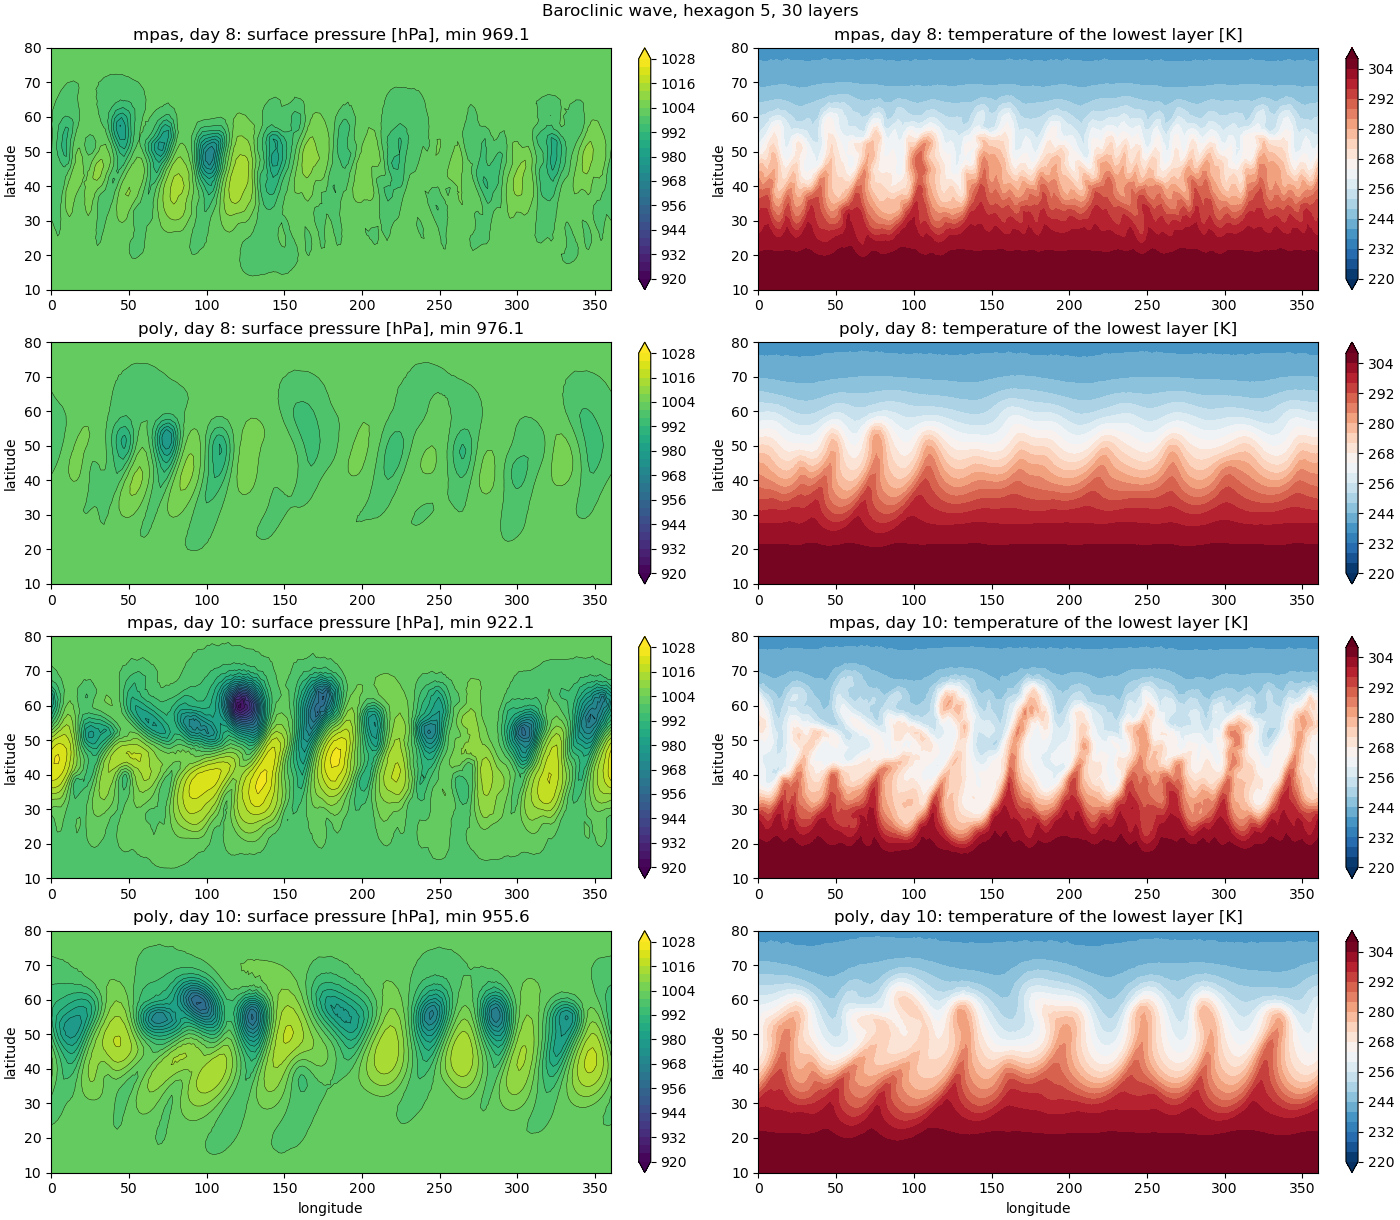
\includegraphics[width=\textwidth]{figures/poly_baroclinic.png}
\caption{Baroclinic wave (Ullrich et al.\ 2014) on hexagon 5 with 30 layers, surface pressure and
temperature of the lowest layer at days 8 and 10: MPAS-Gassmann (\code{mpas}) and \code{PolyEuler}
(\code{poly}), from \code{baroclinic\_wave.jl --out} and \code{examples/plot\_surface.py}.}
\label{fig:baroclinic}
\end{figure}

%==============================================================================
\section{Tests and examples}

\begin{table}[h]
\centering\small
\begin{tabular}{p{0.3\textwidth}p{0.62\textwidth}}
\toprule
test set (\code{test/polyhedral.jl}) & checks \\
\midrule
cell complexes and the integration of monomials & exact moments (cube, prism, non-convex prism), divergence theorem, closure and volume of spherical shells, non-planar faces \\
polynomial reconstruction and transport & polynomials reproduced up to degree 3, tangential basis, mass to round-off, order 4 of the steady transport with degree 3 \\
interaction regions and shallow water & exactness of \code{G}, \code{T} for linear fields, cell vectors, Williamson 2 on hexagons and triangles, mass, no allocations, MPI 1 vs.\ 3 ranks bitwise \\
cut cells & closure, terrain faces on the surface, volume, merging, zero flux through the terrain, free stream, mass, order of the steady transport \\
Euler equations & a stratified atmosphere at rest (not the reference) balanced exactly and kept at rest for a day, surface pressure, mass, the layout of the columns \\
\bottomrule
\end{tabular}
\end{table}

Run with \code{julia +1.12 --project=. test/runtests.jl} (or include \code{test/polyhedral.jl}).
The MPI subtest starts \code{mpiexec} with the repository environment, which needs an instantiated
\code{Manifest.toml} for that Julia version (\code{Pkg.instantiate()}); MPI.jl then uses its own MPICH
unless \code{LocalPreferences.toml} selects a system MPI through \code{MPIPreferences}.

\begin{table}[h]
\centering\small
\begin{tabular}{ll}
\toprule
\code{examples/polyhedral/} & \\
\midrule
\code{galewsky\_poly.jl} & Galewsky jet, MPI and GPU, Figure~\ref{fig:galewsky} \\
\code{mountain.jl} & Euler equations over a hill on cut cells, Figure~\ref{fig:mountain} \\
\code{figure\_data.jl} & data of Figures~\ref{fig:meshes}--\ref{fig:cut} \\
\code{plot\_doc.py}, \code{plot\_mountain.py} & the figures (matplotlib) \\
\code{../baroclinic\_wave.jl poly}, \code{../plot\_surface.py} & baroclinic wave, Figure~\ref{fig:baroclinic} \\
\bottomrule
\end{tabular}
\end{table}

\end{document}
